%!BIB program=biber

\documentclass[10pt,aspectratio=169]{beamer} %类型为文章
\usepackage[UTF8]{ctex} %中文编码宏
\usepackage{multicol} %分栏控制宏
\usepackage{hyperref} %超链接宏
\usepackage{lastpage} %总计页的宏
\usepackage{color} %颜色控制宏
\usepackage{graphicx} %图片插入宏
\usepackage{subfigure} %子图插入宏
\usepackage{animate} %动画插入宏
\usepackage{multirow} %纵向合并宏
\usepackage{makecell} %表格换行宏
\usepackage{amsmath} %公式插入宏
\usepackage{cases}
\usepackage{unicode-math} %公式样式宏
\usepackage{gbt7714} %国标引用宏
\usepackage{url} %网页链接宏
\usepackage{doi} %doi号宏
\usepackage{svg}
\usepackage{algorithm2e} %伪代码宏
\renewcommand{\vec}[1]{\boldsymbol{#1}} %设置向量样式

\usetheme{Berlin}
\usecolortheme{beaver}

\linespread{1.2} %行距
\setlength{\parskip}{0.5em} %段落间距
\setlength{\parindent}{2em} %缩进距离

\setmathfont{Cambria Math} %设置数学公式样式
%\bibliographystyle{gbt7714-numerical} %设置参考文献样式

%\logo{
\includegraphics[height=0.1\textwidth]{images/SCU_logo.pdf}}
%\setbeamertemplate{background}{
\includegraphics[height=\paperheight]{images/SCU_logo.pdf}}
\setbeamertemplate{itemize items}{$\blacksquare $}
\setbeamertemplate{caption}[numbered]


\title{相位衍射相位恢复方法} %设置标题
\subtitle{使用多重网格方法加速层叠相干衍射成像}
\author{欧纪阳} %设置作者
\institute[SCU]{\textit{College of Physics, Sichuan University, Chengdu 610064, China}}
\date{\today} %设置日期

\begin{document}
\maketitle %插入标题

\AtBeginSection{
    \begin{frame}
        \frametitle{目录}
        \tableofcontents[currentsection,subsectionstyle=hide]
    \end{frame}
}

\AtBeginSubsection{
    \begin{frame}
        \subsectionpage
    \end{frame}
}

\section{层叠相干衍射成像迭代引擎(PIE)}

\begin{frame}
    \begin{figure}
        \begin{center}
            \subfigure[装置示意图]{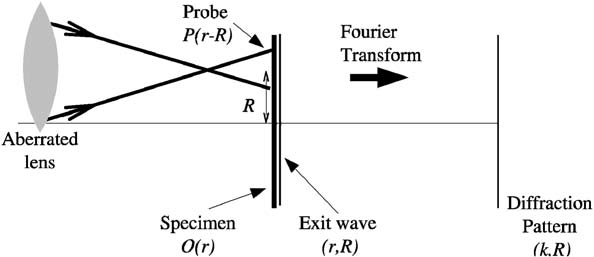
\includegraphics[height=4cm]{images/PIE.png}}
            \quad
            \subfigure[迭代示意图]{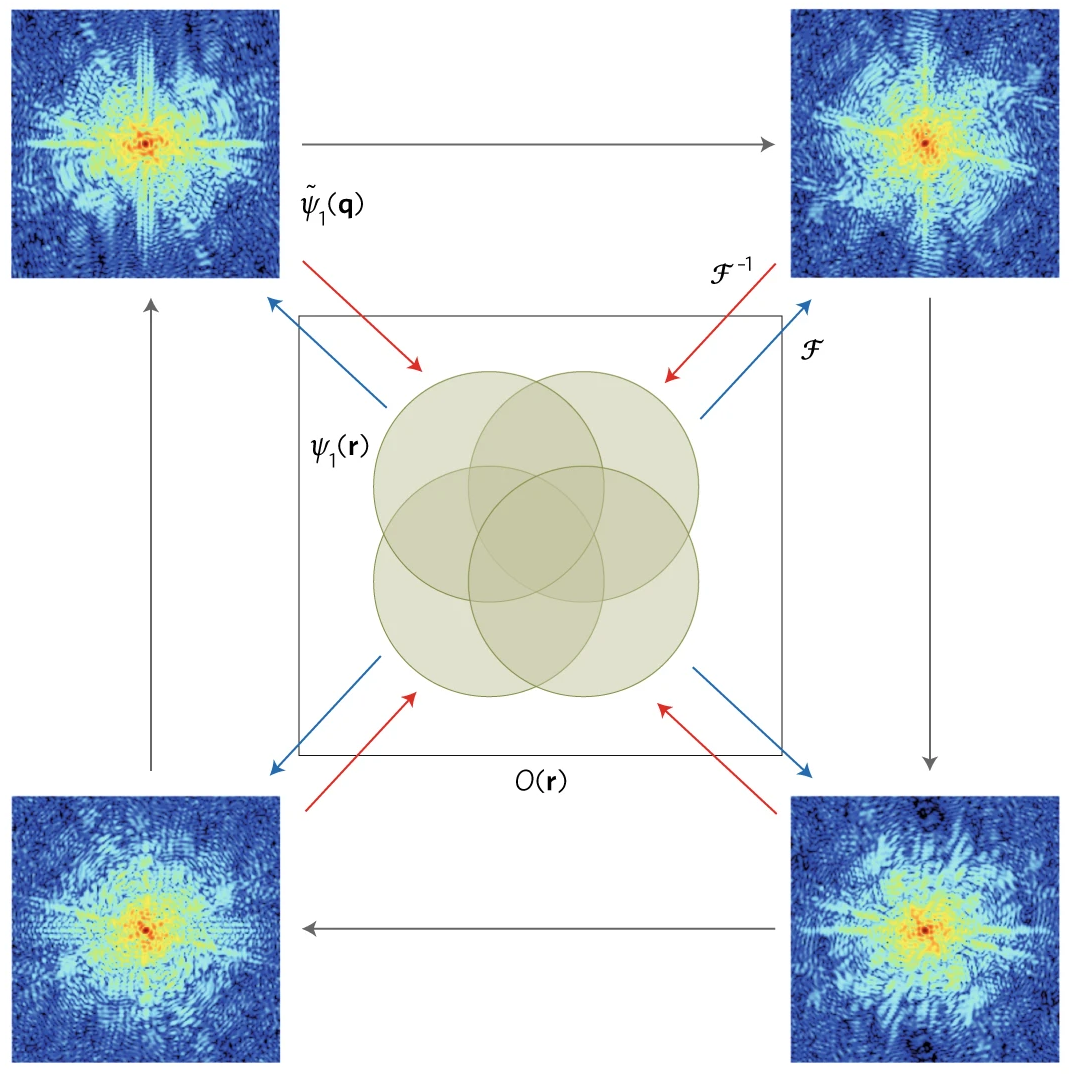
\includegraphics[height=4cm]{images/41566_2017.png}}
        \end{center}
        \qquad 
        \caption{层叠相干衍射成像(Ptychography)}
    \end{figure}
\end{frame}

\begin{frame}[allowframebreaks]
    在照明区域的大小和位置已知的情况下,算法的内循环分为以下几个步骤。首先是给定整个对象区域的振幅和相位一初值$O_0(\vec{r})$,以及照明函数一初值$P_0(\vec{r})$
    \begin{enumerate}
        \item 用对象函数$O_j(\vec{r})$和照明函数$P_j(\vec{r}-\vec{R})$计算出该照明区域的出射波函数,
              \begin{align}
                  \Psi _j(\vec{r},\vec{R})=O_j(\vec{r})P_j(\vec{r}-\vec{R}) \label{0}
              \end{align}
              其中$\vec{R}$为样品与照明区域之间的相对位移。
        \item 对出射函数应用傅里叶变换,并用衍射图案的测量值替代计算值,
              \begin{align*}
                  F_j(\vec{k}) & =\mathcal{F}\{\Psi _j(\vec{r})\} & F_j'(\vec{k}) & =|F_{je}(\vec{k})|\cdot \frac{F_j(\vec{k})}{|F_j(\vec{k})|}
              \end{align*}
              其中$|F_{je}(\vec{k})|$是指照射第$j$个照明区域所产生的衍射图案的测量值。
        \item 应用傅里叶逆变换并做适当的约束,得到更新后的出射波函数,
              \begin{align*}
                  \Psi _{j}'(\vec{r}) & =\mathcal{F}^{-1}\{F_j'(\vec{k})\} & \Psi _{j}''(\vec{r}) & =C[\Psi _{j}'(\vec{r})]
              \end{align*}
              其中$C$函数指的是约束函数,也可以是无约束。
        \item 用更新后的出射波函数拆分得到对象函数的更新函数,
              \begin{align}
                  O_{j+1}(\vec{r}) & =O_{j}(\vec{r})+\alpha \left(\frac{|P_j(\vec{r}-\vec{R})|^2}{[P_j(\vec{r}-\vec{R})]_{MAX}^2} \frac{P_j^*(\vec{r}-\vec{R})}{|P_j(\vec{r}-\vec{R})|^2+\beta}\right)[\Psi _{j}''(\vec{r})-\Psi _{j}(\vec{r})] \label{1}
              \end{align}
              或(ePIE)得到对象函数和照明函数的更新函数,
              \begin{align*}
                  O_{j+1}(\vec{r}) & =O_{j}(\vec{r})+\alpha_O \frac{P_j^*(\vec{r}-\vec{R})}{|P_j(\vec{r}-\vec{R})|_{MAX}^2}[\Psi _{j}''(\vec{r})-\Psi _{j}(\vec{r})] \\
                  P_{j+1}(\vec{r}) & =P_{j}(\vec{r})+\alpha_P \frac{O_j^*(\vec{r}+\vec{R})}{|O_j(\vec{r}+\vec{R})|_{MAX}^2}[\Psi _{j}''(\vec{r})-\Psi _{j}(\vec{r})]
              \end{align*}
    \end{enumerate}
\end{frame}

\subsection{更新函数的权重表示}

\begin{frame}
    考虑最简单的更新函数,由(\ref{0})可得:
    \begin{align}
        O_{j+1}(\vec{r}) = \frac{\Psi _j''(\vec{r})}{P_j(\vec{r}-\vec{R})} = \frac{P_j^*(\vec{r}-\vec{R})}{|P_j(\vec{r}-\vec{R})|^2} \Psi _j''(r) \label{1.1}
    \end{align}
    显然上式对于(\ref{1.1})式对于在照明强度较弱的情况下条件较差,应该更多的保留之前对于对象函数的估计,于是可以在更新时加上一定的权重:
    \begin{align*}
        O_{j+1}(\vec{r}) & = (1-w_j)O_j(\vec{r}) + w_j \frac{P_j^*(\vec{r}-\vec{R})}{|P_j(\vec{r}-\vec{R})|^2} \Psi _j''(r)                        \\
                         & = O_{j}(\vec{r}) + w_j \frac{P_j^*(\vec{r}-\vec{R})}{|P_j(\vec{r}-\vec{R})|^2}[\Psi _{j}''(\vec{r})-\Psi _{j}(\vec{r})]
    \end{align*}
\end{frame}

\begin{frame}
    \begin{align*}
        O_{j+1}(\vec{r}) = O_{j}(\vec{r}) + w_j \frac{P_j^*(\vec{r}-\vec{R})}{|P_j(\vec{r}-\vec{R})|^2}[\Psi _{j}''(\vec{r})-\Psi _{j}(\vec{r})]
    \end{align*}
    其中$w_j$由
    \begin{align*}
        w_j=\alpha \frac{|P_j(\vec{r}-\vec{R})|^2}{|P_j(\vec{r}-\vec{R})|_{MAX}^2}
    \end{align*}
    给出,表示第$j$个照明区域的更新权重,于是可以得到对象函数的更新函数:
    \begin{align*}
        O_{j+1}(\vec{r}) =O_{j}(\vec{r})+\alpha \frac{P_j^*(\vec{r}-\vec{R})}{|P_j(\vec{r}-\vec{R})|_{MAX}^2}[\Psi _{j}''(\vec{r})-\Psi _{j}(\vec{r})]
    \end{align*}
\end{frame}

\subsection{更新函数的梯度表示}

\begin{frame}
    考虑以下的误差度量:
    \begin{align*}
        E_j^O = \frac{1}{2} \sum _{\vec{r}} |O_j(\vec{r})P_j(\vec{r}-\vec{R})-\Psi _j''(\vec{r})|^2
    \end{align*}
    PIE算法的目标是找到一个修正的对象函数$O_j(\vec{r})$,来降低该误差,使出射波$O_j(\vec{r})P_j(\vec{r}-\vec{R})$更接近于算法中更新的出射波$\Psi _j''(\vec{r})$,该误差相对于对象函数的梯度为:
    \begin{align*}
        \nabla E_j^O = \frac{\partial E_j^O}{\partial O_j(\vec{r})} = P_j^*(\vec{r}-\vec{R}) [O_j(\vec{r})P_j(\vec{r}-\vec{R})-\Psi _j''(\vec{r})]
    \end{align*}
    由于误差是在该梯度方向上增加的,因此可以在负梯度方向上将对象函数移动一个小步长$\gamma$来减小误差:
    \begin{align*}
        O_{j+1}(\vec{r}) = O_{j}(\vec{r}) - \gamma \nabla E_j^O = O_{j}(\vec{r}) + \gamma P_j^*(\vec{r}-\vec{R}) [\Psi _j''(\vec{r}) - \Psi _j(\vec{r})]
    \end{align*}
\end{frame}

\begin{frame}
    \begin{align*}
        O_{j+1}(\vec{r}) = O_{j}(\vec{r}) + \gamma P_j^*(\vec{r}-\vec{R}) [\Psi _j''(\vec{r}) - \Psi _j(\vec{r})]
    \end{align*}
    其中$\gamma$设置为
    \begin{align*}
        \gamma=\frac{\alpha}{|P_j(\vec{r}-\vec{R})|_{MAX}^2}
    \end{align*}
    当$\alpha \leq 1$时,步长是稳定的,且对于凸问题收敛性是保证的,但是梯度下降方法收敛缓慢,且收敛缓慢,易停滞在局部极小值处,而PIE更新函数的每次应用使对象函数朝着不同方向的梯度移动,因此可以很好的避免这个问题。
    \begin{align*}
        O_{j+1}(\vec{r}) =O_{j}(\vec{r})+\alpha \frac{P_j^*(\vec{r}-\vec{R})}{|P_j(\vec{r}-\vec{R})|_{MAX}^2}[\Psi _{j}''(\vec{r})-\Psi _{j}(\vec{r})]
    \end{align*}
    
    
\end{frame}

\section{PIE基于梯度的最优化问题}

\subsection{投影最优化问题}

\begin{frame}[allowframebreaks]
    层叠相干衍射成像可以描述为:
    \begin{align*}
        \vec{d}_k & =|\mathcal{F} (\hat{Q}_k \vec{z})|^2+\epsilon_k, & k=1,2,\cdots ,N
    \end{align*}
    其中$\vec{z}$是重建对象,$\vec{d}_k$表示第$k$个扫描位置对应的衍射图案测量值,$\hat{Q}_k$为照明矩阵(探针),即表示第$k$次扫描的位置。考虑强度的高斯误差度量:
    \begin{align*}
        \Phi _{\mathcal{IG}}(\vec{z})=\frac{1}{2}\sum_k^N \left\lVert |\mathcal{F}(\hat{Q}_k \vec{z})|^2 -\vec{d}_k \right\rVert _2^2
    \end{align*}
    定义测量约束集,以及其投影算子分别为:
    \begin{align*}
        \mathcal{M}_k (\vec{z}) & =\left\{\vec{z} : |\mathcal{F}(\hat{Q}_k \vec{z})|^2=\vec{d}_k\right\}, & \mathcal{PM}_k (\vec{z}) & =\mathcal{F}^{-1} \left[\sqrt{\vec{d}_k}\odot \exp{(i \theta \mathcal{F}(\hat{Q}_k \vec{z}))}\right]
    \end{align*}
    则PIE对应的投影最优化问题可以表示为:
    \begin{align}
         & \min \limits_z \Phi (\vec{z}), & \Phi (\vec{z}) & =\frac{1}{2}\sum_k^N \left\lVert \mathcal{PM}_k(\vec{z})-\hat{Q}_k \vec{z} \right\rVert _2^2 \label{2}
    \end{align}
    即寻找$\vec{z}$使上式右侧达到最小值或者0。
    
    那么PIE迭代过程中的(\ref{1})式用以上的表示方法可以写为:
    \begin{align}
        \vec{z}(\vec{r}) & =\vec{z}(\vec{r})+\alpha \left(\frac{\hat{Q}_k}{[\hat{Q}_k]_{MAX}} \frac{\hat{Q}_k^T}{|\hat{Q}_k|^2+\beta}\right)[\mathcal{PM}_k(\vec{z})-\hat{Q}_k \vec{z}] \label{3}
    \end{align}
    其中$\hat{Q}_k^T$表示$\hat{Q}_k$的复共轭转置。
\end{frame}

\subsection{梯度下降方法}

\begin{frame}
    \begin{algorithm}[H]
        \LinesNumbered
        \SetKwFunction{f}{f}
        \SetKwFunction{g}{g}
        \KwIn{\f{$x$}:目标函数,$x_0$:初始预测值,$\lambda$:检索步长$\varepsilon$:计算精度
        }
        \For{$k=0,1,2,\cdots$}{
            $g_k$=\g{$x_k$}=$\nabla$\f{$x_k$}\\
            \eIf{$\left\Vert g_k \right\Vert < \varepsilon$}{
                $x^*$=$x_k$
            }{
                $x_{k+1}$= $x_k-\lambda g_k$
            }
        }
        \KwOut{$\varphi$:线性方程组的解}
        \caption{\small 梯度下降方法}
        \label{A1}
    \end{algorithm}
\end{frame}

\begin{frame}
    考虑(\ref{2})式的梯度:
    \begin{align}
        \nabla  \Phi (\vec{z}) = \frac{\partial \Phi (\vec{z})}{\partial \vec{z}} = \sum_k^N \hat{Q}_k [\mathcal{PM}_k(\vec{z})-\hat{Q}_k^T \vec{z}]
    \end{align}
    PIE迭代的内循环(即对所有的$N$个照明区域都做(\ref{3})式),在基于梯度的最优化问题中可以表示为:
    \begin{align}
        \vec{z}=\vec{z}-\gamma \nabla \Phi (\vec{z})
    \end{align}
    即在每一次外循环中,PIE等价于向负梯度方向移动了一个小步长。
\end{frame}

\section{PDE中的多重网格方法}

\subsection{基础算法构成}

\begin{frame}
    在数值分析中,多重网格法是一种使用层次离散化来求解微分方程的方法,是多分辨率方法的一个例子。由于直接在高分辨率(用于求解的间隔小)上进行求解时对于低频部分收敛较慢,与间隔的平方成反比,便想可以到先在低分辨率(间隔较大)上进行求解,然后再进行插值,提高其分辨率,再在更高分辨率进行计算,这样的方法就叫做多重网格方法,且迭代过程主要包含以下几个重要的组成部分:
    \begin{itemize}
        \item 平滑(smoothing):用线性求解器进行迭代,降低高频误差。
        \item 计算残差(Residual Computation):在平滑之后计算剩余误差(残差)$r_i=b-Ax_i$。
        \item 限制(Restriction):降低采样率,把残差放到更加粗糙的网格中。
        \item 延拓(prolongation):将粗网格计算的修正值插值到更精细的网格中
        \item 修正(Correction):将延拓的修正值添加到精细网格中。
    \end{itemize}
\end{frame}

\begin{frame}
    \footnotesize
    \begin{algorithm}[H]
        \LinesNumbered
        \KwIn{$\varphi$:初始预测值,$f$:常数项,$h$:最精细网格精度,$h_m$:最粗糙网络精度
        }
        \SetKwFunction{VCycle}{VCycle}
        \SetKwFunction{smoothing}{smoothing}
        \SetKwFunction{residual}{residual}
        \SetKwFunction{restriction}{restriction}
        \SetKwFunction{prolongation}{prolongation}
        \SetKwFunction{zeros}{zeros}
        \SetKwFunction{size}{size}
        \SetKwProg{Fn}{Function}{:}{end}
        \Fn{\VCycle{$\varphi,f,h$}}{
            $\varphi$ = \smoothing{$\varphi,f,h$} '预平滑(pre-smoothing)\\
            $res$ = \residual{$\varphi,f,h$}\\
            $rhs$ = \restriction($res$)\\
            $eps$ = \zeros(\size($rhs$))\\
            \eIf{$h$ < $h_m$}{
                \VCycle{$eps,rhs,2h$}
            }{
                \smoothing{$eps,rhs,2h$}
            }
            $\varphi$ = $\varphi$ + \prolongation($eps$)\\
            $\varphi$ = \smoothing{$\varphi,f,h$} '后平滑(post-smoothing)\\
            \textbf{return} $\varphi$
        }
        \KwOut{$\varphi$:方程的解}
        \caption{\small $\nabla^2 \varphi=f$的V循环多重网格方法}
        \label{A2}
    \end{algorithm}
\end{frame}

\begin{frame}
    \begin{figure}
        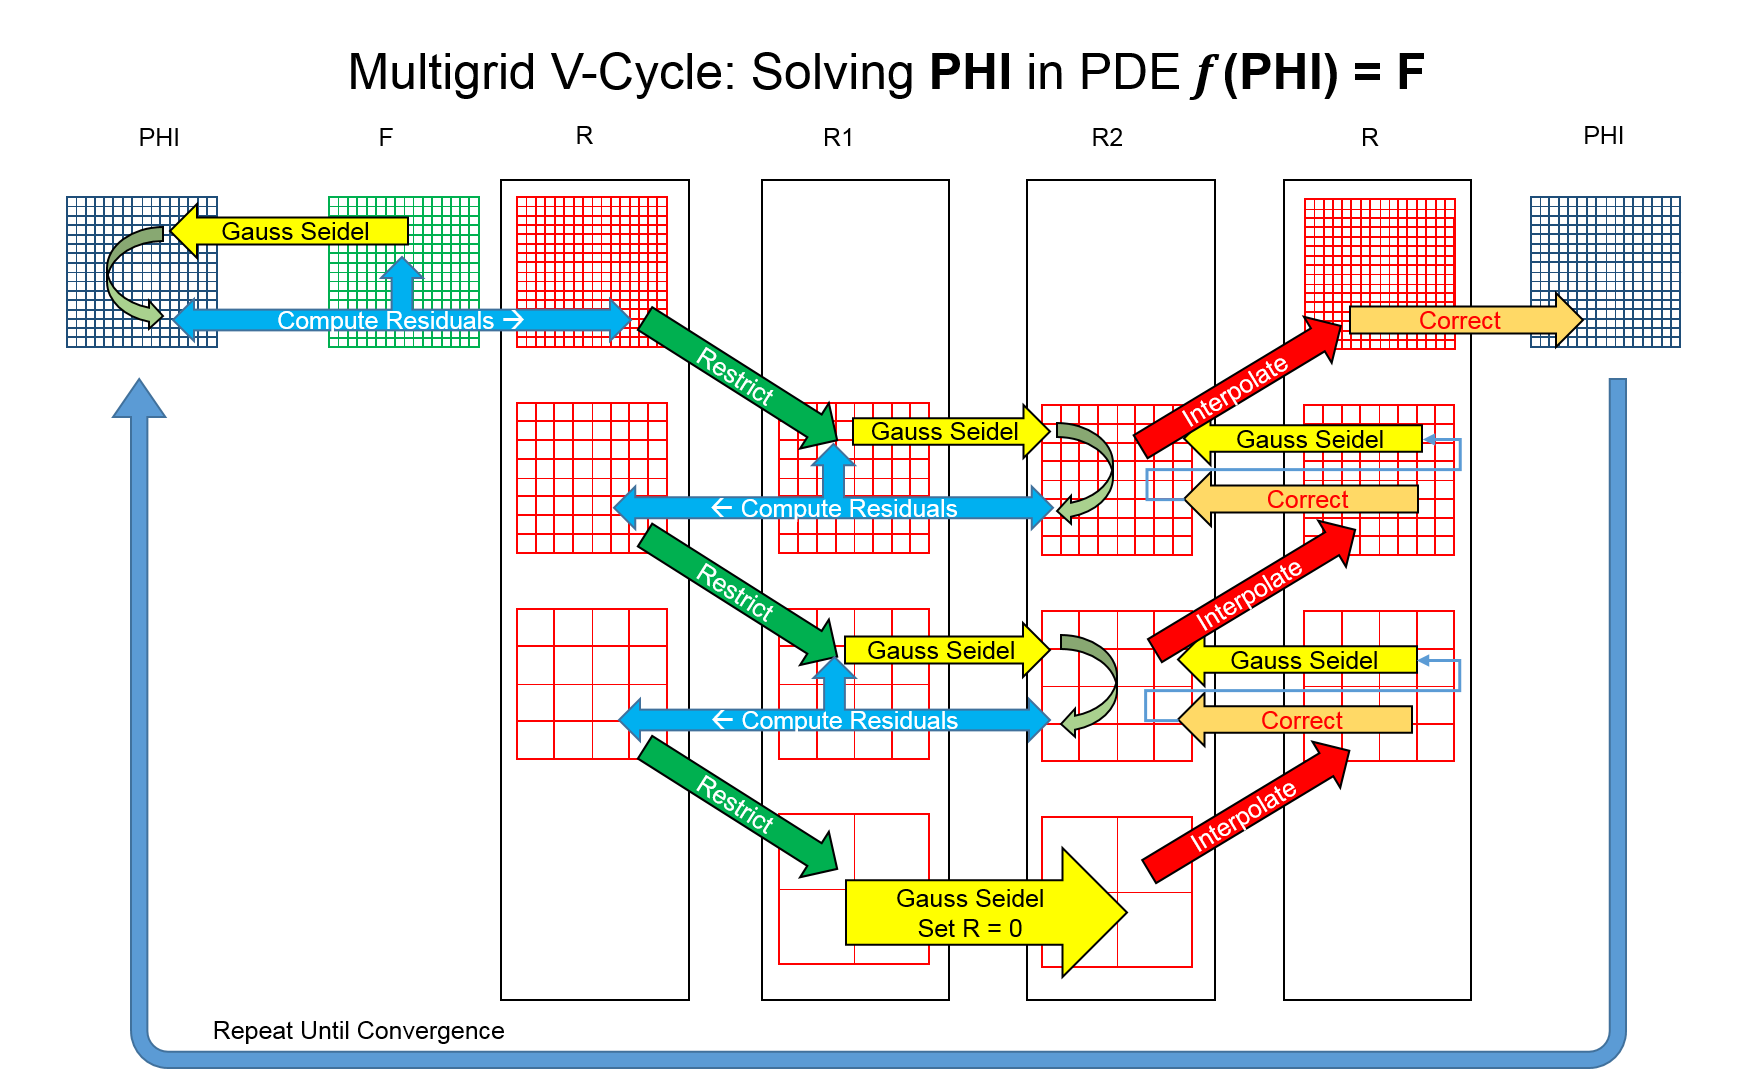
\includegraphics[height=6cm]{images/Multigrid_Visualization.png}
        \caption{V循环多重网格方法的示意图}
    \end{figure}
\end{frame}

\begin{frame}
    \begin{figure}
        \includesvg[height=5.5cm]{images/MultigridWork.svg}
        \caption{三种多重网格方法的迭代图}
    \end{figure}
\end{frame}

\subsection{求解泊松方程的举例}

\begin{frame}
    利用多重网格-五点差分-共轭梯度法和直接共轭梯度方法(只在一级网格中进行迭代)分别对(\ref{3.1a})式进行求解,设置求解区域为$S=\left\{(x,y)|-1\leq x\leq 1,-1\leq y\leq 1\right\}$的正方形区域,边界条件设置为(\ref{3.1b})(\ref{3.1c})式,在两个维度上的网格精度均为$10^{-3}$,即求解区域的网格大小为$2000\times 2000$,
    \begin{subnumcases}{}
        \frac{\partial^2 \varphi}{\partial x^2}+\frac{\partial^2 \varphi}{\partial y^2}=-\frac{\rho}{\varepsilon}=-2\pi^2 \sin(\pi x)\sin(\pi y) \label{3.1a}\\
        \varphi=0, \, x=\pm 1 \label{3.1b} \\
        \varphi=0, \, y=\pm 1 \label{3.1c}
    \end{subnumcases}
    该系统具有解析解,并可推导得到电场强度矢量的表达式,
    \begin{align*}
        \varphi & =\sin(\pi x)\sin(\pi y) & E=-\pi\cos(\pi x)\sin(\pi y)\vec{e_x}+\pi\sin(\pi x)\cos(\pi y)\vec{e_y}
    \end{align*}
\end{frame}

\begin{frame}
    \begin{figure}
        %\includegraphics[height=6cm]{images/q2e.png}
        \caption{多重网格-五点差分-共轭梯度法的求解结果}
    \end{figure}
\end{frame}

\begin{frame}
    \begin{figure}
        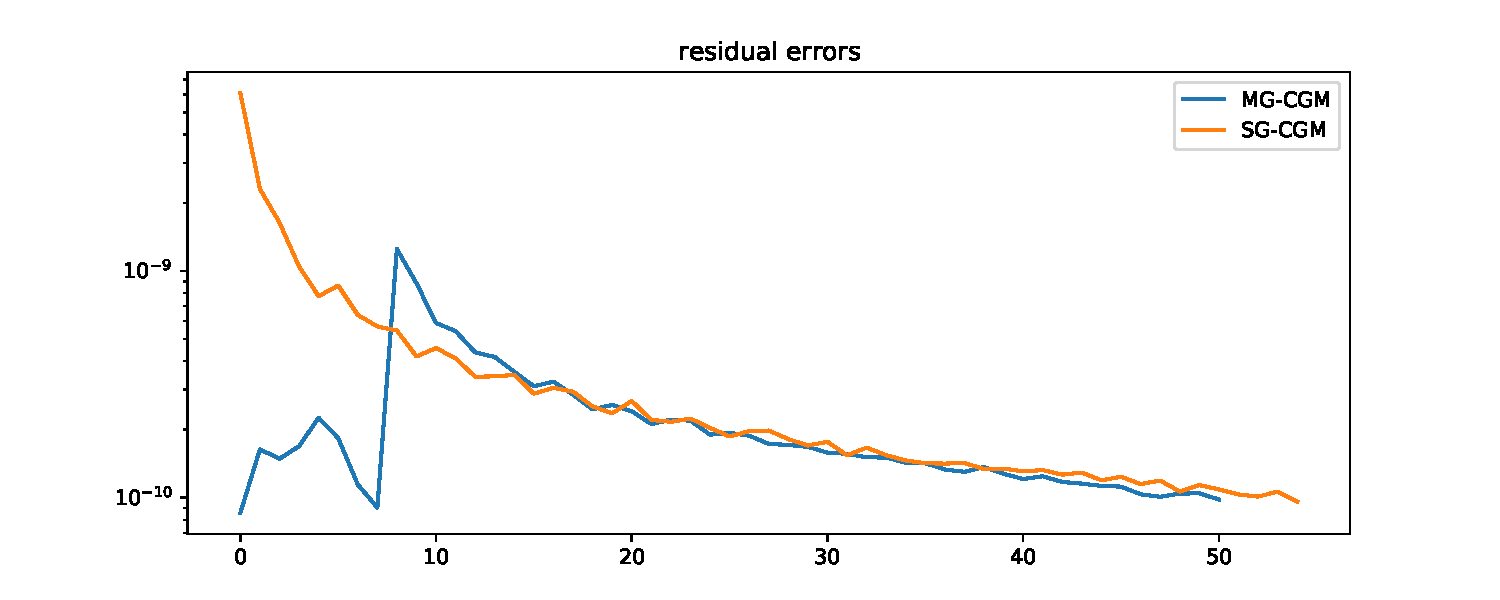
\includegraphics[height=4.8cm]{images/error.pdf}
        \begin{flushleft}
            \footnotesize \qquad 多重网格法的后平滑迭代过程在三级网格中经历了1次,在二级网格中经历了7次,在一级网格中经历了43次,平均总计耗时6.89692s;直接共轭梯度法经历55次迭代,平均总计耗时10.2639s。
        \end{flushleft}
        \caption{两种算法的误差下降曲线}
    \end{figure}
\end{frame}

\section{多重网格框架与PIE的结合}

\begin{frame}
    \frametitle{为什么要将两者进行结合}
    \begin{itemize}
        \item CDI中的相位恢复问题可以看做是最优化问题,多重网格框架可以用于解决此类问题;
        \item 目前的傅里叶迭代算法易出现收敛到局部最小值,而无法收敛到全局最小值的情况;
        \item 在CDI实验中,可以轻松提取出不同频段成分;
        \item 在CDI算法中,高频部分与低频率部分的收敛速度往往不尽相同;
        \item 对粗糙网格进行处理,计算成本低廉收敛迅速,插值后可作为精细网格的预测。
    \end{itemize}
    

\end{frame}

\end{document}